% Section 2. Review method. Rewritten 2026-10-20 (session 0839c9f4) for the state after the search update, the
% subscription databases, full-text tranche T1, the re-check tranche R797 and the screening freeze D0051; the census
% subsections are kept from the 2026-10-15 draft. Every count has a % src comment; flow counts come from
% analysis/prisma/prisma-flow.json (script analysis/prisma/prisma_flow.py) unless stated.
\section{Review method}
\label{sec:method}

\paragraph{The method at a glance.} Three identification strands (a curated seed corpus, a search update over free sources and six subscription databases) fed one screening pipeline: two independent automated screeners per record, an adjudicator for disagreements, fixed written criteria, and verbatim quotes matched against each paper. Screening was frozen on 2026-10-20 with 615 included studies. RQ1 counts use fields recorded for all 615; RQ2 to RQ6 use a stratified random sample of 80 studies, extracted with a fixed form and appraised on nine quality items; a census of a random sample of seed records codes the value rule behind each headline result. The section ends with the departures from the protocol; the full list is in the Supplement (Section~S1), and Section~\ref{sec:limits} states what each does to the conclusions.

\subsection{Design, reporting standard and protocol status}
\label{sec:method-design}

The review is reported against PRISMA~2020~\cite{page2021prisma} (checklist in the supplement, Section~S1) and follows Kitchenham and Charters' procedure for systematic reviews in computing~\cite{kitchenham2007guidelines}. The protocol (research questions, eligibility, sources, selection, extraction, appraisal, synthesis) is archived with the data and code (version~0.1 of 2026-10-13). % src: research/review/protocol.md header line "DRAFT v0.1, 2026-10-13; not frozen"
It was \emph{not} frozen or registered before screening: the freeze rule asked for a git tag after sign-off, and none exists. % src: protocol.md "Freeze rule"; `git tag` returned no tags on 2026-10-15
Amendments are recorded in protocol section~10 and in a decision ledger with one row per decision (identifiers D0001 onwards, cited below); Section~\ref{sec:method-deviations} lists every departure. % src: protocol.md section 10; research/ledgers/decisions.jsonl

\subsection{Information sources and searches}
\label{sec:method-sources}

The search ran in three strands (Table~\ref{tab:sources}; Figure~\ref{fig:prisma}). The \emph{seed corpus} joined a curated list of diffusion language model papers with two logged arXiv searches of 2026-10-14. The \emph{search update} of 2026-10-15 ran revised strings on five free sources and snowballed citations from the seed; the strings were revised after the protocol's recall pilot failed, and the final strings kept seed recall at 525 of 540. The \emph{subscription strand} searched six databases on 2026-10-15 and 2026-10-16 through institutional access. Every query, date and hit count is logged; the strings, the recall checks and the export limits are in the Supplement (Section~S1).

\begin{table}[t]
\caption{Sources searched and records identified, before deduplication. Counts from the search log and the merge statistics; the full strings are in the supplement (Section~S1).}
\label{tab:sources}
\small
\begin{tabular}{@{}p{5.1cm}p{2.9cm}r@{}}
\toprule
Source & Date & Records \\
\midrule
\multicolumn{3}{@{}l}{\emph{Seed corpus}} \\
Awesome-DLMs list (commit 194aa6bd) & parsed 2026-10-13 & 572 \\ % src: prisma-flow.json seed.identified_awesome_dlms
arXiv API, strings S1 and S2 & 2026-10-14 & 1,331 \\ % src: prisma-flow.json seed.identified_arxiv_S1 1158 + S2 173
\multicolumn{3}{@{}l}{\emph{Search update (strings S1, S2, S1$'$, S2$'$)}} \\
Semantic Scholar bulk API & 2026-10-15 & 10,572 \\ % src: prisma-flow.json free.identified_databases_by_source
arXiv API & 2026-10-15 & 6,105 \\
OpenReview API & 2026-10-15 & 3,357 \\
OpenAlex & 2026-10-15 & 1,081 \\
ACL Anthology & 2026-10-15 & 355 \\
Citation searching, backward and forward & 2026-10-15 & 45,421 \\ % src: free.identified_citation_searching (19423 + 25998)
\multicolumn{3}{@{}l}{\emph{Subscription databases}} \\
Scopus & 2026-10-15 & 4,046 \\ % src: prisma-flow.json subscription.identified_by_database
SpringerLink & 2026-10-16 & 2,614 \\
Web of Science Core Collection & 2026-10-15 & 2,267 \\
IEEE Xplore & 2026-10-15 & 1,300 \\
ScienceDirect & 2026-10-16 & 613 \\
ACM Digital Library & 2026-10-15 & 329 \\
\midrule
Total identified & & 79,964 \\ % src: 1903 + 66891 + 11169 (fig01-prisma.log seed_id, upd_id; subscription.identified)
\bottomrule
\end{tabular}
\end{table}

\paragraph{Deduplication and automation filters.} Records were merged on shared identifiers and normalised titles, leaving 1,453 seed records, 19,328 new update records and 4,380 new subscription records. The final strings were then applied locally and excluded 17,486 update and 4,201 subscription records by automation; a validation of that filter crossed its preset reversal threshold, so a single-screener rescue pass read every filtered record with an abstract (Supplement, Section~S1).

\subsection{Eligibility}
\label{sec:method-eligibility}

A record is included if it satisfies all of the following. It proposes, analyses, evaluates or benchmarks (a) a diffusion model, in discrete or continuous state space, whose output includes natural-language text or code, or (b) a unified model, one model and not a pipeline, that both understands and generates across text and at least one other modality (image, video, audio or speech, or 3D) with a diffusion, masked-generative or discrete-flow component. It is a primary study with a method, theory or empirical result. Its full text is in English, and its first public version is dated 2021-01-01 or later. % src: protocol.md section 2 (I1 to I4) and section 10 (I1(b) amendment, decision D0020)
Exclusions carry one code: X0 no diffusion component, X1 non-text diffusion not covered by (b), X2 text only as conditioning, X3 secondary study, X4 no method, theory or result, X5 duplicate, X6 full text unavailable, X7 application of an unchanged model with no model-level finding, X8 outside the date window or not English. % src: screening/criteria-v1.6-screener.md; decision D0032
Full-text screening applied criteria v1.6, which fixes the order in which codes are tried and how a diffusion component is recognised; it was revised through five red-team audits before the first full-text decision. % src: decision D0032; research/review/audits/2026-10-16-redteam-criteria-v1.1.md to -v1.5.md

\subsection{Selection process and agreement}
\label{sec:method-screening}

\paragraph{Title and abstract.}
Two automated screeners (see the Declaration on the use of AI) read each record independently from fixed written criteria, blind to each other; a record passed to full text if either marked it include or unclear (decision D0030). % src: decision D0030; screening/v2/SCREENER-BRIEF.md
In the seed strand the two screeners agreed on pass against exclude for 1,333 of 1,453 records ($\kappa=0.728$)~\cite{cohen1960coefficient}. % src: tools/screening_agreement.py output (2026-10-15): "pass-to-full-text agree 0.917 kappa 0.728"; screener-B/run-log.jsonl
In the update and subscription strands they agreed with $\kappa=0.911$ (95\% bootstrap interval 0.892 to 0.929) on 1,953 records, and $\kappa=0.930$ (0.861 to 0.985) on the first 246 of 260 subscription records, the other 14 agreeing in every case. % src: analysis/screening/agreement-v2.log ("pass vs exclude raw 0.955 kappa 0.911 [0.892, 0.929]"); screening/v2/dual-subscription/agreement-sub.json (n 246, kappa 0.9302 [0.8614, 0.9852]), agreement-sub-02.json (10 of 10), agreement-sub-03.json (4 of 4)
1,243 seed records, 954 update records and 52 subscription records passed. % src: prisma-flow.json seed.ta_pass_either, free.ta_pass_D0030, subscription.ta_pass_D0030

\paragraph{Full text.}
Full texts were retrieved from open-access sources or through the institutional e-gateway, logged and hashed, converted to text with page markers, and checked against the record's title. % src: research/review/fulltext/fetch-log.jsonl; analysis/screening/ft-t1/t1-provenance.jsonl; tools/ft_title_check.py
Each batch of about ten records went to screener~A and screener~B in separate dispatch folders that held only the criteria, the batch's texts and an output file. Every decision had to cite verbatim evidence with its page; a script checked each quote against the text and returned an unmatched quote to its screener once. Disagreements, ``adjudicate'' rows and quotes still unmatched went to an adjudicator, who saw both rows. % src: criteria-v1.6.md section 4 items 1-5; tools/ft_dispatch.py; quote_check.py; analysis/screening/c-run-log.jsonl (route F line, 2026-10-16)
Each session's transcript was checked for reads outside its folder and for the model that produced every turn; a session that failed either check was discarded and rerun. % src: tools/ft_isolation_check.py; tools/ft_model_check.py; research/progress.md HANDOFF 18 (t1b081 B rerun)
Tranche T1 assessed the update and subscription passes: 885 reports, all decided, 608 included and 277 excluded (X0 77, X1 103, X2 85, X3 7, X4 4, X7 1); the adjudicator ruled on 116, and 3 of the exclusions are the records screener~B could not read (below). Before adjudication, A and B agreed on pass against exclude with $\kappa=0.894$ (0.859 to 0.927; $n=882$). % src: prisma-flow.json full_text_T1 (decided_incl_resolved 885, include_incl_resolved 608, exclude_incl_resolved 277, exclude_codes_incl_resolved, adjudicated_by_C 116, kappa 0.8939 [0.8589, 0.9268]); analysis/screening/agreement-ft-t1.json; decisions D0058, D0059
208 reports were not retrieved (Figure~\ref{fig:prisma}). % src: fig01-prisma.log t1_not_retrieved
For three biology papers and, later, one more, screener~B's sessions failed and their rows were discarded. For these four records the first author confirmed screener~A's reading (three exclusions X1 in T1, one X2 in R797); they have no independent second screening and are left out of every agreement statistic (decisions D0041, D0046, D0056, D0058). % src: decisions D0041, D0046, D0056, D0058; analysis/screening/b-unavailable-resolved.jsonl; prisma-flow.json full_text_T1.resolved_B_unavailable_D0058, full_text_R797.resolved_B_unavailable_D0058

\paragraph{Re-check of title and abstract exclusions.}
Because most title-and-abstract exclusions in the update rested on one model, 797 exclusions were flagged by preset rules as possible errors, a random 100 of them were screened at full text, together with 32 further records found by a keyword query. The preset rule sent all 797 to full text if any sampled record was included; 4 of the 82 sampled records screened were included, so the rule fired. % src: criteria-v1.6.md section 5.1-5.3; analysis/screening/ta-recheck-k.json (K 4: M03416, M10984, R0963, R1202; included 4, excluded 78, not_in_T1 18)
The remaining 715 formed tranche R797, screened as T1 until the freeze: 285 reports assessed and decided, 7 included and 278 excluded; agreement before adjudication was $\kappa=0.602$ (0.362 to 0.793) with raw agreement 0.961 and Gwet's AC1 0.957, the low $\kappa$ reflecting how few records passed. % src: prisma-flow.json full_text_R797; analysis/screening/agreement-ft-r797.json (n 284)

\paragraph{Human validation.}
The protocol asks a human author to screen a random 15\% of each full-text tranche blind and requires each model screener to reach $\kappa\ge0.70$ against that author. For T1 two of the authors read the 108-record sample without recording per-record decisions (decision D0034; authors' statement of 2026-10-20); the R797 sample of 108 was drawn before any download and was not screened before the freeze. After the analysis the first author checked three blind random samples instead, validated as described in the Declaration on the use of AI (decisions D0065, D0066). On 40 T1 records (20 included and 20 excluded by the models) the author and the final decision agree on 21 of the 30 both decided ($\kappa=0.41$, 95\% interval 0.09 to 0.71; 10 unclear; the exclusion code matches on all 11 joint exclusions), below the protocol's 0.70 and on fewer than its 100 records. On 12 extraction records the study-level flags agree in 31 of 34 pairs ($\kappa=0.82$), and on 24 census papers the value-rule class agrees for 21 ($\kappa=0.79$; Supplement~S9). Every other screening statistic above is agreement between two models. % src: decisions D0034, D0035, D0048, D0065, D0066; screening/human-validation-t1/sample-manifest.json; human-validation-r797/sample-manifest.json; analysis/screening/human-check-screening-agreement.json; analysis/extraction/d0052/human-check-agreement.json; analysis/census/human-check-census-agreement.json


\begin{figure}[p]
\centering
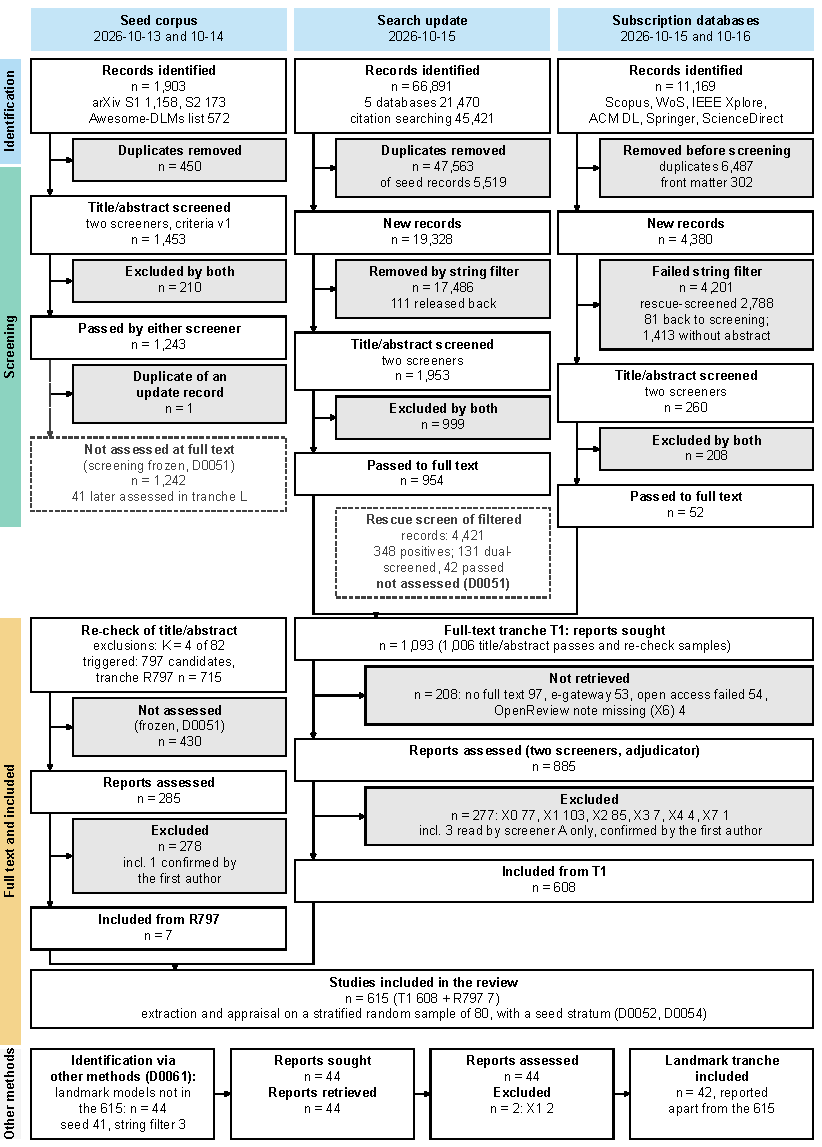
\includegraphics[width=\linewidth]{figures/fig01-prisma.pdf} % src: paper/review/scripts/fig01_prisma.py; every count read from analysis/prisma/prisma-flow.json, sums asserted, log figures/fig01-prisma.log
\caption{PRISMA 2020 flow. Three identification strands are screened separately and meet at full text. Grey boxes are records removed or excluded; dashed boxes are sets identified but not assessed at full text when screening was frozen (decision D0051). ``Awaiting second screener'' marks records that screener~B could not read and that the first author screens. X0 to X7 are exclusion codes (Section~\ref{sec:method-eligibility}). The bottom row is the landmark tranche, identified by other methods after the freeze (decision D0061).}
\label{fig:prisma}
\Description{A flow diagram in three columns. The seed corpus (1,903 records from a curated list and two arXiv searches) is deduplicated to 1,453 and screened by title and abstract; 1,243 pass, and 1,242 of these are not assessed at full text when screening was frozen (41 of them are assessed later in the landmark tranche). The search update identifies 66,891 records, of which 19,328 are new; a string filter removes 17,486; 1,953 are screened and 954 pass. The subscription databases identify 11,169 records, 4,380 new; 260 are screened and 52 pass. The update and subscription passes form full-text tranche T1: 1,093 reports sought, 208 not retrieved, 885 assessed, 277 excluded and 608 included. A re-check of title-and-abstract exclusions found 4 inclusions among 82 sampled records, which triggered tranche R797 of 715 records; 285 were assessed before the freeze and 7 included. In total 615 studies are included. A bottom row shows a landmark tranche identified by other methods: 44 papers of design-space models not in the 615, all retrieved and assessed, 42 included and 2 excluded, reported apart from the 615.}
\end{figure}

\subsection{Screening freeze}
\label{sec:method-freeze}

On 2026-10-20 the authors stopped screening to finish the review with the resources available (decision D0051). Three sets were identified but not screened at full text: the 1,242 seed records that passed title and abstract, the 430 R797 records not yet reached, and the 348 positives of the update's rescue pass (131 of them dual-screened, 42 passing). % src: decision D0051; prisma-flow.json not_screened_D0051 (seed_tranche_S1243_D0037.frame 1242, R797_remainder 430, free_source_rescue_positives_D0036)
The included set is therefore 615 studies (608 from T1 and 7 from R797): 596 from the search update, 13 from the subscription databases and 6 seed records that reached full text through the re-check of title-and-abstract exclusions. The seed records that passed title and abstract, which include widely used models such as LLaDA, MDLM, Dream and MMaDA, are therefore outside the screened set. To keep that strand in the evidence, the extraction sample adds a random seed stratum drawn from the census sample, whose full-text eligibility was judged by the census coders (Section~\ref{sec:method-extraction}; decision D0054). Section~\ref{sec:limits} discusses what the freeze does to each research question. % src: analysis/rq1/rq1-counts.json (n 615, by_tranche); rq1-includes.jsonl id prefixes M 596, U 13, R 6; research/progress.md HANDOFF 27 (R0128, R0205, R0246, R0350 in S1243); decision D0054
\paragraph{Landmark tranche.} After the freeze, the papers of the 44 design-space models (Section~\ref{sec:design}) that are not among the 615 were screened as a targeted tranche, identified by other methods (decision D0061): 41 unscreened seed records and 3 snowball records that the string filter had removed. All 44 full texts were retrieved and screened under criteria v1.6 by the same two screeners, who agreed on every include or exclude decision: 42 were included and 2 excluded (X1). A seeded random order of the 42 was fixed before extraction, and the first 16 were extracted with the same form and procedure as the sample until the compute budget was spent (decision D0063). The tranche is reported in its own column and changes neither the 615 nor any estimate for them. % src: analysis/screening/landmark/landmark-frame-summary.json (tranche_L 44; S1243 41, other 3); analysis/prisma/prisma-flow.json landmark_tranche_D0061 (identified 44, reports_retrieved 44, assessed 44, include 42, exclude 2, exclude_codes X1 2, agreement_A_B 44, adjudicated_by_C 0); analysis/extraction/lmk/extraction-order.json (seed 20261024, N 42); rq-results.json D0060 landmark_meta n_extracted 16; decisions D0061, D0063

\subsection{Data extraction and quality appraisal}
\label{sec:method-extraction}

\paragraph{All included studies (RQ1).}
For all 615 included studies the counts for RQ1 come from fields the screeners recorded at full text: the eligibility basis (I1(a), I1(b) or both), the modality, whether text is produced, the research questions the study bears on, and the year. Where the two screeners recorded different values the record is counted as split. % src: analysis/rq1/rq1_counts.py docstring; rq1-counts.json
\paragraph{Stratified sample (RQ2 to RQ6).} Evidence for RQ2 to RQ5 and the quality appraisal (RQ6) come from a stratified random sample of 80 studies (decisions D0051, D0052, D0054). Three strata cover the included studies: unified multimodal studies, and language-only studies split at the median text length into shorter and longer ones (52, 267 and 265 studies after later field resolutions; 59 sampled). A fourth stratum of 20 seed-corpus studies, drawn from those the census found eligible, is reported apart, as is the landmark tranche (decisions D0060, D0063). Shares are weighted to the stratum sizes, with 95\% bootstrap intervals; the estimator was chosen after extraction. The form (153 fields) records each paper's own comparisons as matched groups with their arms, metric, direction and budget, and nine appraisal items, QA1 to QA9: code, weights or data, evaluation protocol, run-to-run variation, uncertainty for the main comparison, baselines at matched or reported budget, an ablation of the credited component, claims that agree with the paper's own tables, and stated limitations. One automated extractor read each study and cited a page for every value; a validator checked every value against the text; a second extractor read 8 studies, and an adjudicator settled their differences from the full text. The two extractors agree on the values (616 of 616) and metric directions (75 of 76) of the contrast units both found and on most appraisal scores and study-level flags, but on only 5 of 8 direction flags, and they cut the same tables into comparison groups very differently (36 of 245 groups found by both, F1 0.29). Section~\ref{sec:rq} therefore draws no unit totals and makes its statements about studies. Twenty-seven records kept an entry the validator rejected; Supplement~S6 repeats the estimates without them. The full procedure is in the Supplement (Section~S4).

\paragraph{Synthesis.}
RQ2 to RQ5 are answered with a verdict (well supported, mixed, weakly supported or untested; protocol section~7) under thresholds stated in Section~\ref{sec:rq}. RQ1 and RQ6 are described. The abstract claim types (CT1 to CT6) are taken from the earlier claim-evaluability rubric and reported descriptively, because the synergy type did not reach reliability there. No meta-analytic pooling was attempted: the protocol's threshold of comparable contrasts on the same task, metric and budget is not met. % src: protocol.md section 7; research/review/feasibility/stage2/summary-*.md

\subsection{Census: sampling, coding and adjudication}
\label{sec:census-method}

The census of Section~\ref{sec:census} predates the search update and samples the seed corpus only; its eligibility judgements used the protocol's rules as amended on 2026-10-15 (decision D0020), not criteria v1.6. The pool is the 1,106 seed records that both title-and-abstract screeners passed and that have an arXiv identifier, put in a random order (seed 20261015) before coding; ranks 1 to 176 were coded, of which 4 have no full text, 5 are ineligible and 167 eligible. Two automated coders, blind to each other, coded the headline result, the value rule behind it (field F2) and four reporting fields; agreement was computed under codebook v1.1 before reconciliation, and adjudicators applied codebook v1.2, written afterwards. One possible leak of one coder's labels into the other's workspace is reported. The full procedure, with the stopping rule, codebook versions, adjudication counts and the incident, is in the supplement (Section~S3). % src: census-result-v2.md ("Sample", "Process", "Limits"); tools/census_sample.py (SEED 20261015); coverage/census-codebook-v1.md, -v1.1.md, -v1.2.md; decisions D0015, D0019, D0020, D0021

\subsection{Departures from the protocol}
\label{sec:method-deviations}

Twelve departures from the protocol are listed with their decision numbers in the Supplement (Section~S1). They fall into three groups. \emph{Protocol status:} the protocol was not registered before screening; the search strings were revised after a failed recall pilot; and the verdict definitions and thresholds, the estimator and the primary population were fixed after the results were known (Section~\ref{sec:rq} reports how far the verdicts depend on them). \emph{Selection:} screening was frozen before three identified sets were assessed, among them the seed corpus with the most-cited models (Section~\ref{sec:method-freeze}); the planned human validation was replaced by later author checks (Section~\ref{sec:method-screening}); and a few records were settled by the first author confirming an automated reading. \emph{Extraction and synthesis:} extraction covers a stratified sample of 80 studies by one extractor, with a second on 8; a claim-evaluability extension was suspended; the census codebook was amended after coding; the appraisal was run on the sample only; a landmark tranche was screened after the freeze and reported apart; and the comparability table, dose--response curves and appraisal by year and venue that the protocol promised are not given.

